\title{
		02257 Applied Functional Programming\\
	----- Project 3 -----
	}
\author{
Casper Sloth Paulsen (s110448)\hspace{1cm}
\includegraphics[scale=.2]{csp.png}\\
Stefan Mertens (s113420)\hspace{1cm}
\includegraphics[scale=.1]{stm.png}\\
Anders Rydbirk (s113725)\hspace{1cm}
\includegraphics[scale=.35]{ar.png}
}
\date{\today}

\documentclass[12pt]{article}
\usepackage[T1]{fontenc} % the font encoding
\usepackage[utf8]{inputenc} % the input encoding
\usepackage{lmodern} % the Latin Modern font
\usepackage{graphicx}
\usepackage{geometry}
\usepackage{listings}
\usepackage{color}
\usepackage{epstopdf}
\usepackage{xcolor}

\definecolor{bluekeywords}{rgb}{0.13,0.13,1}
\definecolor{greencomments}{rgb}{0,0.5,0}
\definecolor{turqusnumbers}{rgb}{0.17,0.57,0.69}
\definecolor{redstrings}{rgb}{0.5,0,0}
\definecolor{dkgreen}{rgb}{0.0,0.35,0}
\definecolor{dred}{rgb}{0.545,0,0}
\definecolor{dblue}{rgb}{0,0,0.545}
\definecolor{lgrey}{rgb}{0.9,0.9,0.9}
\definecolor{gray}{rgb}{0.4,0.4,0.4}
\definecolor{darkblue}{rgb}{0.0,0.0,0.6}

\lstdefinelanguage{FSharp}{
      backgroundcolor=\color{black!5},  
      basicstyle=\small \ttfamily \color{black} \bfseries,   
      breakatwhitespace=false,       
      breaklines=true,               
      captionpos=b,                   
      commentstyle=\color{dkgreen},   
      deletekeywords={...}, 
      escapeinside={\%*}{*)},                  
      frame=single,                  
      language=TeX, 
      morekeywords={let, new, match, with, rec, open, module, namespace, type, of, member, 			and, for, in, do, begin, end, fun, function, try, mutable, if, then, else},
    keywordstyle=\color{bluekeywords},
    sensitive=false,
    morecomment=[l][\color{greencomments}]{///},
    morecomment=[l][\color{greencomments}]{//},
    morecomment=[s][\color{greencomments}]{{(*}{*)}},
    morestring=[b]",
    stringstyle=\color{redstrings},			%Insert missing keywords here
      emphstyle=\color{cyan},               
      keywordstyle=\color{blue}, 
      identifierstyle=\color{redstrings},
      stringstyle=\color{blue},      
      numbers=none,                 
      numbersep=5pt,                   
      rulecolor=\color{black},        
      showspaces=false,               
      showstringspaces=false,        
      showtabs=false,                
      stepnumber=1,                   
      tabsize=4,
      columns=fullflexible,                
      title=\lstname
}
\geometry{
 a4paper,
 total={210mm,297mm},
 left=25mm,
 right=25mm,
 top=5mm,
 bottom=20mm,
 }

\begin{document}
\clearpage\maketitle
\thispagestyle{empty}

\section{Status}
The status of the project is that it works on the entire abstract syntax tree from project 2. The implementation is capable of generating valid PostScript which is readable in Adobe Acrobat X. It is possible to test the program from the Script.fsx. 

\section{Input types}
The first part of the program, which is an implementation of the SML program, is capable of working on all input types, because it has been made generic. 

\begin{verbatim}
type Tree<'a> =  Node of 'a * (Tree<'a> list)
\end{verbatim}

\section{Extensions/Additions}
We have made the following extensions to the program. 

Initially the program used string appending, but was later converted to returning a list of strings. By returning a list of string it was now possible to make a more efficient implementation for generating the PostScript string. We ended up concluding that String.concat and StringBuilder are more or less equal when it comes to performance, however normal string appending is really slow. This is seen Figure \ref{string_performance}.

\begin{figure}[h]
\begin{verbatim}
1 elem = 1 QuickSortV1 parse tree

Concat 10 elem: Real: 00:00:00.001, CPU: 00:00:00.015, 
GC gen0: 0, gen1: 0, gen2: 0
Naive string append 10 elem: Real: 00:00:01.629, CPU: 00:00:02.281, 
GC gen0: 44, gen1: 30, gen2: 25
StringBuilder 10 elem: Real: 00:00:00.001, CPU: 00:00:00.000, 
GC gen0: 0, gen1: 0, gen2: 0
 
Concat 100 elem: Real: 00:00:00.007, CPU: 00:00:00.000, 
GC gen0: 0, gen1: 0, gen2: 0
Naive string append 100 elem: Real: 00:02:57.580, CPU: 00:04:18.781, 
GC gen0: 2242, gen1: 2225, gen2: 2224
StringBuilder 100 elem: Real: 00:00:00.012, CPU: 00:00:00.015, 
GC gen0: 1, gen1: 1, gen2: 0
\end{verbatim}
\caption{String appending performance}
\label{string_performance}
\end{figure}

\begin{figure}
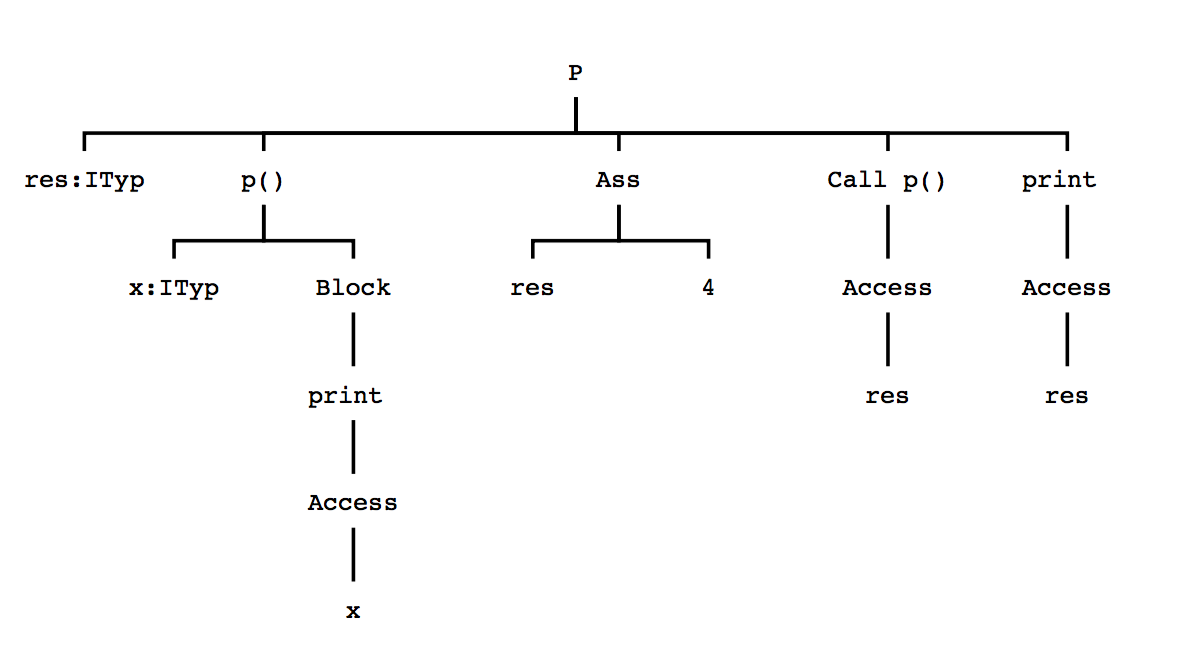
\includegraphics[scale=0.75]{ex1.png}
\caption{A parse tree visualized by our program (Ex1.gc)}
\label{fig:fig2}
\end{figure}

The problem of overlapping labels was solved using substrings. This means that we have hardcoded a maximum length a string can have. Beyond that the excess part of the string is truncated. This solves the problem in a naive way, because a more optimal way was to somehow calculate how long the longest label is and then take that into account when setting the horizontal distance between nodes for the PostScript string.

\section{Reflection}
The beauty (see figure \ref{fig:fig2}) of working with a tree structure is that it is really easy to apply a recursive program on the data structure and mutable state is generally avoided. That is what we have learned from working with this functional pearl.

We have also concluded in general that converting written functional program in one language to another functional program is rather easy, because the paradigm is the same and the general structure can be reused.

In general we found this project really fun and exciting. 


\end{document}